\documentclass{article}
\usepackage[margin=1in]{geometry}
\usepackage{amsmath,amsthm,amssymb}
\usepackage{bbm,enumerate,mathtools}
\usepackage{tikz,pgfplots}
\usepackage{chessboard}
\usepackage[hidelinks]{hyperref}
\usepackage{multicol} % Problem 35

\newenvironment{question}{\begin{trivlist}\item[\textbf{Question.}]}{\end{trivlist}}
\newenvironment{note}{\begin{trivlist}\item[\textbf{Note.}]}{\end{trivlist}}
\newenvironment{references}{\begin{trivlist}\item[\textbf{References.}]}{\end{trivlist}}
\newenvironment{related}{\begin{trivlist}\item[\textbf{Related.}]\end{trivlist}\begin{enumerate}}{\end{enumerate}}


\begin{document}
\rating{2}{3}
A snail travels along the grid in unit steps---but it hates crossing its
trail, so if a step is going to cross is trail, it will only go half way.
\begin{figure}[!h]
  \centering
  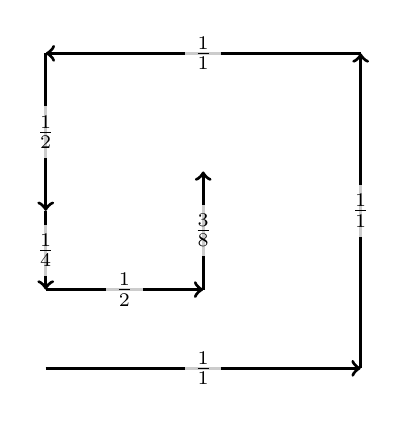
\begin{tikzpicture}[scale=4]
    \draw[very thick, ->] (0,0)--(1,0) node [midway, fill=white, opacity=0.8, text opacity=1] {$\frac{1}{1}$};
    \draw[very thick, ->] (1,0)--(1,1) node [midway, fill=white, opacity=0.8, text opacity=1] {$\frac{1}{1}$};
    \draw[very thick, ->] (1,1)--(0,1) node [midway, fill=white, opacity=0.8, text opacity=1] {$\frac{1}{1}$};
    \draw[very thick, ->] (0,1)--(0,1/2) node [midway, fill=white, opacity=0.8, text opacity=1] {$\frac{1}{2}$};
    \draw[very thick, ->] (0,1/2)--(0,1/4) node [midway, fill=white, opacity=0.8, text opacity=1] {$\frac{1}{4}$};
    \draw[very thick, ->] (0,1/4)--(1/2,1/4) node [midway, fill=white, opacity=0.8, text opacity=1] {$\frac{1}{2}$};
    \draw[very thick, ->] (1/2,1/4)--(1/2,5/8) node [midway, fill=white, opacity=0.8, text opacity=1] {$\frac{3}{8}$};
  \end{tikzpicture}\hspace{1cm}
  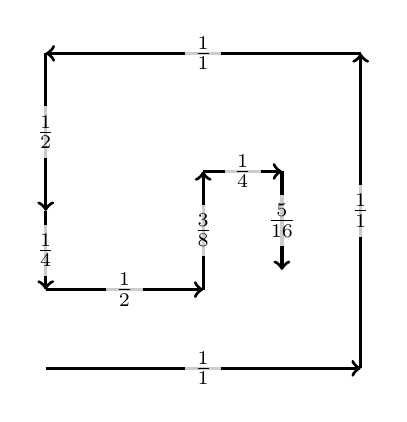
\begin{tikzpicture}[scale=4]
    \draw[very thick, ->] (0,0)--(1,0) node [midway, fill=white, opacity=0.8, text opacity=1] {$\frac{1}{1}$};
    \draw[very thick, ->] (1,0)--(1,1) node [midway, fill=white, opacity=0.8, text opacity=1] {$\frac{1}{1}$};
    \draw[very thick, ->] (1,1)--(0,1) node [midway, fill=white, opacity=0.8, text opacity=1] {$\frac{1}{1}$};
    \draw[very thick, ->] (0,1)--(0,1/2) node [midway, fill=white, opacity=0.8, text opacity=1] {$\frac{1}{2}$};
    \draw[very thick, ->] (0,1/2)--(0,1/4) node [midway, fill=white, opacity=0.8, text opacity=1] {$\frac{1}{4}$};
    \draw[very thick, ->] (0,1/4)--(1/2,1/4) node [midway, fill=white, opacity=0.8, text opacity=1] {$\frac{1}{2}$};
    \draw[very thick, ->] (1/2,1/4)--(1/2,5/8) node [midway, fill=white, opacity=0.8, text opacity=1] {$\frac{3}{8}$};
    \draw[very thick, ->] (1/2,5/8)--(3/4,5/8) node [midway, fill=white, opacity=0.8, text opacity=1] {$\frac{1}{4}$};
    \draw[very thick, ->] (3/4,5/8)--(3/4,5/16) node [midway, fill=white, opacity=0.8, text opacity=1] {$\frac{5}{16}$};
  \end{tikzpicture}\\~\\
  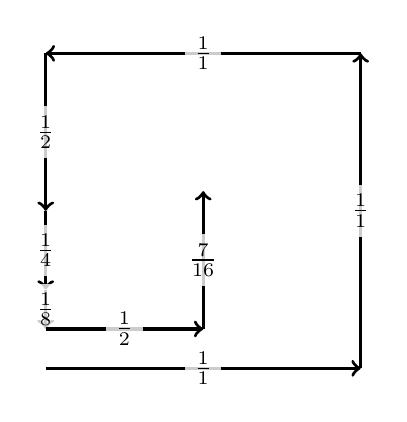
\begin{tikzpicture}[scale=4]
    \draw[very thick, ->] (0,0)--(1,0) node [midway, fill=white, opacity=0.8, text opacity=1] {$\frac{1}{1}$};
    \draw[very thick, ->] (1,0)--(1,1) node [midway, fill=white, opacity=0.8, text opacity=1] {$\frac{1}{1}$};
    \draw[very thick, ->] (1,1)--(0,1) node [midway, fill=white, opacity=0.8, text opacity=1] {$\frac{1}{1}$};
    \draw[very thick, ->] (0,1)--(0,1/2) node [midway, fill=white, opacity=0.8, text opacity=1] {$\frac{1}{2}$};
    \draw[very thick, ->] (0,1/2)--(0,1/4) node [midway, fill=white, opacity=0.8, text opacity=1] {$\frac{1}{4}$};
    \draw[very thick, ->] (0,1/4)--(0,1/8) node [midway, fill=white, opacity=0.8, text opacity=1] {$\frac{1}{8}$};
    \draw[very thick, ->] (0,1/8)--(1/2,1/8) node [midway, fill=white, opacity=0.8, text opacity=1] {$\frac{1}{2}$};
    \draw[very thick, ->] (1/2,1/8)--(1/2,9/16) node [midway, fill=white, opacity=0.8, text opacity=1] {$\frac{7}{16}$};
  \end{tikzpicture}\hspace{1cm}
  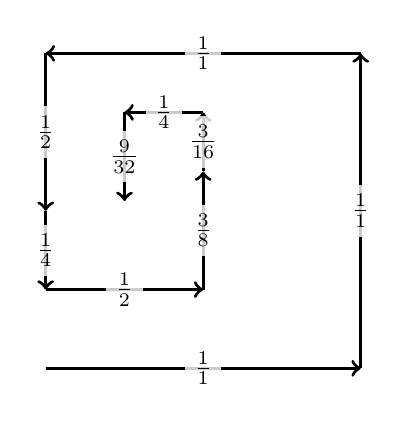
\begin{tikzpicture}[scale=4]
    \draw[very thick, ->] (0,0)--(1,0) node [midway, fill=white, opacity=0.8, text opacity=1] {$\frac{1}{1}$};
    \draw[very thick, ->] (1,0)--(1,1) node [midway, fill=white, opacity=0.8, text opacity=1] {$\frac{1}{1}$};
    \draw[very thick, ->] (1,1)--(0,1) node [midway, fill=white, opacity=0.8, text opacity=1] {$\frac{1}{1}$};
    \draw[very thick, ->] (0,1)--(0,1/2) node [midway, fill=white, opacity=0.8, text opacity=1] {$\frac{1}{2}$};
    \draw[very thick, ->] (0,1/2)--(0,1/4) node [midway, fill=white, opacity=0.8, text opacity=1] {$\frac{1}{4}$};
    \draw[very thick, ->] (0,1/4)--(1/2,1/4) node [midway, fill=white, opacity=0.8, text opacity=1] {$\frac{1}{2}$};
    \draw[very thick, ->] (1/2,1/4)--(1/2,5/8) node [midway, fill=white, opacity=0.8, text opacity=1] {$\frac{3}{8}$};
    \draw[very thick, ->] (1/2,5/8)--(1/2,13/16) node [midway, fill=white, opacity=0.8, text opacity=1] {$\frac{3}{16}$};
    \draw[very thick, ->] (1/2,13/16)--(1/4,13/16) node [midway, fill=white, opacity=0.8, text opacity=1] {$\frac{1}{4}$};
    \draw[very thick, ->] (1/4,13/16)--(1/4,17/32) node [midway, fill=white, opacity=0.8, text opacity=1] {$\frac{9}{32}$};
  \end{tikzpicture}
  \caption{
    Left-to-right and top-to-bottom: examples of walks that end in step sizes
    that have numberators of 3, 5, 7, and 9.
  }
\end{figure}
\begin{question}
  Let $a(n)$ be the minimum number of steps the snail must take before it can
  take a step of size $(2n-1)/2^k$. What is $a(n)$?
\end{question}
\begin{related}
  \item What if the snail must always turn left or right?
  \item What if the snail is walking on a triangular or hexagonal grid?
  \item What is the set of points the snail can step on after finitely many steps?
  \item How many distinct points can the snail reach after $m$ steps?
\end{related}
\begin{references}
  \item \url{https://math.stackexchange.com/q/2678852/121988}
  \item \url{https://oeis.org/A300444}
\end{references}

\end{document}
